\chapter{Tâche 2 : intelligence des cahiers des charges}\label{chap:tender}
\section{Passage de la preuve au domaine métier}
Un texte correctement extrait peut encore être inutilisable pour préparer une réponse. Le CDC demande une lecture de sa structure : titre, sections, articles, obligations, dates, garanties, annexes et bordereaux. Le \texttt{\detokenize{CDCAnalyzer}} reçoit le \texttt{\detokenize{DocumentResult}} par un adaptateur, construit un \texttt{\detokenize{TenderDocument}}, puis transmet certaines pages candidates au module BOQ. Ce découplage rend possible l'analyse d'un PDF natif et d'une image OCR par le même chemin métier, à condition que les preuves textuelles soient suffisantes.

La hiérarchie n'est pas seulement une présentation. Une obligation sous une annexe technique n'a pas le même contexte qu'une clause administrative. Les modèles \texttt{\detokenize{Section}}, \texttt{\detokenize{Article}}, \texttt{\detokenize{Lot}}, \texttt{\detokenize{Annex}} et \texttt{\detokenize{Requirement}} portent des références source. La composition détecte les titres, assemble les paragraphes, enrichit les exigences et identifie les documents spéciaux. Il s'agit de candidats structurés, pas d'une validation juridique.

\section{Structure : titres, parties, articles et annexes}
Les heuristiques de titres examinent le libellé et sa numérotation. Le travail de développement a montré deux échecs précis : les titres arabes \emph{al-fasl} n'étaient pas identifiés comme articles, et des titres «~Lot~» numérotés étaient confondus avec des sections. La révision V2 ajoute des indices multilingues observés dans le corpus, reconnaît les «~Partie I/II~» comme niveaux supérieurs et garde les lots dans une collection distincte. Le résultat est meilleur sur les annotations de développement examinées au \autoref{chap:evaluation}, sans preuve de généralisation à tous les formats arabes ou à tout OCR.

Les annexes sont repérées en préservant le numéro de page physique. La page reste centrale : elle permet à l'interface d'ouvrir le passage correspondant et à l'évaluateur de comparer les localisations. Pour les champs d'identité, une case vide du modèle documentaire reste manquante ; le logiciel ne crée ni date limite de soumission ni référence d'appel d'offres à partir du contexte voisin.

\begin{figure}[htbp]\centering
\begin{tikzpicture}[every node/.style={font=\small,align=center},box/.style={draw=ink,rounded corners,fill=pale,minimum width=26mm,minimum height=9mm},arr/.style={-{Latex},draw=espritred,thick},node distance=8mm]
\node[box] (root) {Dossier CDC};
\node[box,below left=of root] (part) {Partie};
\node[box,below right=of root] (ann) {Annexe};
\node[box,below=of part] (art) {Article};
\node[box,left=of art] (lot) {Lot};
\node[box,below=of art] (req) {Exigence candidate};
\draw[arr] (root)--(part);\draw[arr] (root)--(ann);\draw[arr] (part)--(art);\draw[arr] (part)--(lot);\draw[arr] (art)--(req);
\end{tikzpicture}
\caption{Hiérarchie simplifiée du modèle CDC ; les lots restent distincts des sections.}\label{fig:hierarchie}
\end{figure}

\section{Exigences, délais et données financières}
Le module d'exigences classe des phrases candidates selon des motifs d'obligation et le contexte des articles ou annexes. Une simple recherche du verbe «~doit~» manquerait des variantes et confondrait parfois citation et obligation ; les indices structuraux apportent le contexte, sans résoudre tous les cas linguistiques. Les résultats ne sont pas exhaustifs : sur 26 exemples de faits positifs annotés, 14 sont retrouvés. Une évaluation limitée aux seuls exemples positifs ne donne ni précision ni rappel exhaustif du composant. Les faits financiers et temporels utilisent une normalisation de nombres, dates et durées. Le code maintient un lien entre la version accentuée de la source et la chaîne pliée utilisée pour la recherche ; cette correspondance d'offsets corrige un défaut où les extraits bruts perdaient leur place après normalisation.

L'interface de revue laisse un fait à l'état \texttt{\detokenize{unreviewed}}, \texttt{\detokenize{approved}} ou \texttt{\detokenize{corrected}}, avec une correction explicite et un horodatage. Le résultat machine et sa preuve demeurent distincts de la décision humaine. Cette séparation est nécessaire pour pouvoir dire ce que l'outil a proposé et ce qu'un analyste a choisi ; elle rejoint les principes de conception d'interactions humain--IA où l'utilisateur doit pouvoir comprendre et corriger le système \cite{amershi}. Le dépôt ne comporte pas d'identité de relecteur vérifiée ni de contrôle d'accès ; la revue ne constitue donc pas une piste d'audit complète de production.

\section{Détection et extraction des bordereaux}
Un BOQ rassemble des lignes de prestation avec, selon le formulaire, désignation, unité, quantité, prix unitaire, montant et totaux. Une seule règle universelle de colonnes serait séduisante, mais les gabarits changent leurs en-têtes, leurs positions et leurs lignes. Le flux en deux niveaux reconnaît d'abord une page candidate par les indices de titre et d'en-tête, puis tente de reconstruire les lignes. Le parseur spécialisé \texttt{\detokenize{MALE_MUNICIPAL_MAINTENANCE_BOQ_V1}} exploite la géométrie connue du formulaire ministériel. Le parseur \texttt{\detokenize{GENERIC_LAYOUT_BOQ_V1}} cherche des en-têtes sémantiques placés et attribue les fragments de ligne aux colonnes observées. La spécialisation est prioritaire lorsqu'elle correspond ; elle évite de dégrader un format connu par une heuristique plus large, au prix d'une couverture réduite sur d'autres formats.

\begin{figure}[htbp]\centering
\begin{tikzpicture}[every node/.style={font=\small,align=center},box/.style={draw=ink,rounded corners,fill=pale,minimum width=39mm,minimum height=10mm},arr/.style={-{Latex},draw=espritred,thick},node distance=7mm]
\node[box] (a) {Pages candidates CDC};
\node[box,below=of a] (b) {Famille MALE reconnue ?};
\node[box,below left=8mm and 9mm of b] (s) {Colonnes géométriques\\spécialisées};
\node[box,below right=8mm and 9mm of b] (g) {En-têtes et alignements\\génériques};
\node[box,below=24mm of b] (v) {Valeurs brutes, preuves,\\contrôles et absences};
\draw[arr] (a)--(b);\draw[arr] (b)--(s);\draw[arr] (b)--(g);\draw[arr] (s)--(v);\draw[arr] (g)--(v);
\end{tikzpicture}
\caption{Extraction BOQ spécialisée ou générique, suivie de contrôles explicites.}\label{fig:boq-pipeline}
\end{figure}

La reconstruction générique gère dans les tests un en-tête sur deux lignes, une désignation repliée avec conservation des deux preuves, des en-têtes répétés et un libellé de colonne explicitement TTC. La reconnaissance du niveau HT ou TTC vient des mots présents dans l'en-tête, pas d'une hypothèse comptable. Les descriptions très irrégulières, les cellules fusionnées et la continuation multipage sans nouvel en-tête restent hors du domaine validé. Une ligne peut être détectée mais garder des valeurs numériques nulles. Le système ne remplit pas les cases manquantes par déduction.

\begin{table}[htbp]\centering\tighttable
\begin{tabularx}{\textwidth}{@{}p{28mm}Y Y@{}}\toprule
Aspect & Extracteur spécialisé & Extracteur générique\\\midrule
Déclenchement & Famille ministérielle connue & Indices de BOQ + en-tête positionné\\
Colonnes & Géométrie du formulaire & Concepts d'en-tête et positions observées\\
Atout & Stabilité sur la référence connue & Essai de transfert à d'autres gabarits\\
Preuve actuelle & Gabarit réel vide et fixtures synthétiques & Régressions synthétiques positionnées\\
Risque principal & Couverture étroite & Variabilité du tableau et de l'OCR\\\bottomrule
\end{tabularx}
\caption{Portée effective des deux extracteurs BOQ.}\label{tab:boq-comparaison}
\end{table}

\section{Le cas décisif du formulaire vide}
Le PDF réel de référence compte 30 pages et son Annexe 05 se trouve à la page physique 25. Le bordereau y présente cinq emplacements d'articles, numérotés 01 à 05. Les désignations, quantités, prix et montants ne sont pas renseignés. Les contrôles arithmétiques retournent \texttt{\detokenize{NOT_CHECKABLE}} plutôt que \texttt{\detokenize{VALID}} pour les sommes. Cette distinction est fondamentale : le cas vérifie la localisation d'un gabarit et la conservation du vide, mais ne peut servir à calculer la précision des nombres sur des offres achevées. La \autoref{fig:source-boq} reproduit un extrait du document de référence pour rendre l'absence observable.

\begin{figure}[H]\centering
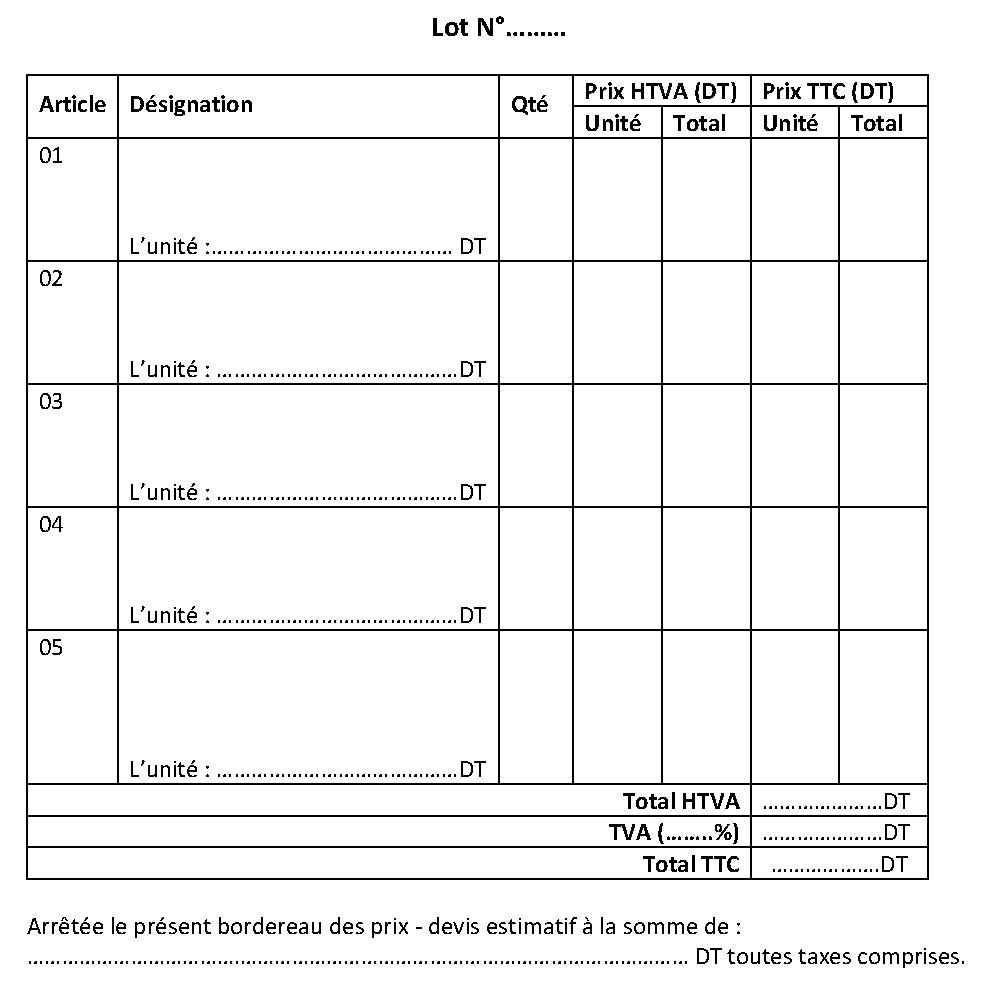
\includegraphics[width=0.70\textwidth]{figures/boq_reference_page25.pdf}
\caption{Extrait authentique de l'Annexe 05 du PDF de référence, page 25 : emplacements de bordereau non remplis.}\label{fig:source-boq}
\end{figure}

La validation compare les montants seulement lorsque quantité et prix existent. Elle emploie des nombres décimaux et une tolérance définie dans le module de contrôle ; une absence devient \texttt{\detokenize{NOT_CHECKABLE}}, une incohérence mesurable peut être signalée. Des fixtures synthétiques testent par exemple un nombre français, une quantité manquante et une erreur de multiplication. Ces cas prouvent le comportement du programme sur des entrées contrôlées, pas sa robustesse sur des offres réelles variées.

\section{Ask Tender : retrouver avant de formuler}
Ask Tender indexe les passages et les faits déjà structurés de \texttt{\detokenize{TenderDocument}} pour répondre à une question. Une génération directe sur le PDF entier rendrait plus difficile l'attribution de la réponse à une page précise. Le système commence donc par retrouver des preuves : la requête est normalisée, les mots fréquents sont réduits et une carte limitée de concepts d'achat public augmente le score de passages déjà observés (délai, garantie, durée, pièces, paiement ou bordereau). Les alias améliorent le classement ; ils ne créent jamais une valeur factuelle. Les résultats sont dédupliqués par élément source et exposent page et preuve. Un chemin déterministe formule certaines réponses courtes ; Ollama peut générer localement depuis les passages sélectionnés, si un modèle est disponible. Ce choix facilite l'audit et l'exécution locale, mais sa récupération lexicale peut manquer une paraphrase nouvelle. En l'absence de modèle local, l'interface signale le repli.

Une citation est une aide à la vérification, pas une garantie automatique de pertinence. Les tests de récupération disponibles portent sur quatre puis sept questions synthétiques revues. La page attendue apparaît dans les trois premiers résultats pour les quatre premières ; pour les sept nouvelles, elle se trouve en première position dans les sept cas. Les textes et la formulation de ces questions étant contrôlés, on ne peut pas extrapoler un taux de bonne réponse en situation réelle.

\begin{figure}[H]\centering
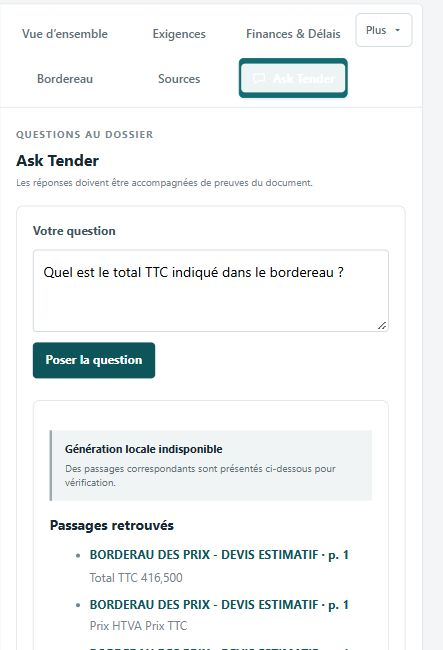
\includegraphics[width=0.53\textwidth]{screenshots/07_ask_detail.jpg}
\caption{Vue réelle d'Ask Tender sur une fixture BOQ synthétique : passages cités et indisponibilité explicite de la génération locale.}\label{fig:ui-ask}
\end{figure}

\section{Persistance, interface et chiffrage}
\begin{figure}[H]\centering
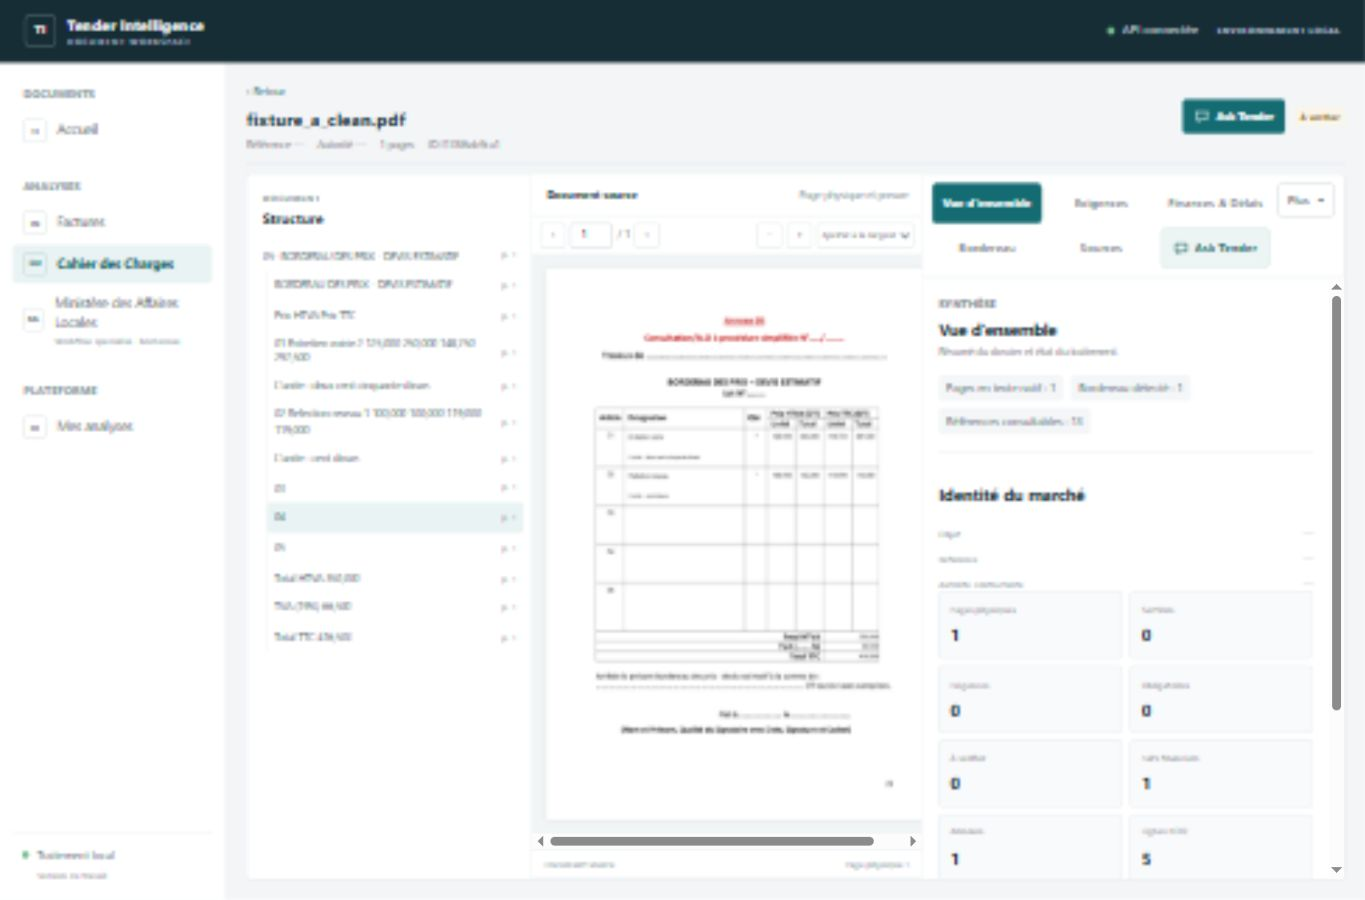
\includegraphics[width=\textwidth]{screenshots/03_workspace.jpg}
\caption{Workspace exécuté localement avec la fixture BOQ synthétique : structure à gauche, document source au centre et analyse à droite.}\label{fig:ui-workspace}
\end{figure}
L'API FastAPI publie les routes d'analyse, de chargement de page, de sauvegarde, de recherche, d'interrogation, de revue et d'export CSV. Le stockage local associe un identifiant opaque à la réponse enregistrée. Le parcours de bibliothèque recherche par nom ou identifiant et rouvre une analyse sans réexécuter le producteur de preuves. Les tests API remplacent même \texttt{\detokenize{DocumentProcessor}} par un composant qui échouerait s'il était rappelé lors de certaines réouvertures. L'interface offre un visualiseur de la source, un espace CDC, un espace BOQ et un brouillon de prix.

Le brouillon de chiffrage ne modifie pas le BOQ extrait. Écraser la valeur source par une saisie corrigerait l'affichage mais détruirait la possibilité de contrôler l'erreur initiale. Pour chaque ligne, le système distingue donc les quantités ou prix lus dans la source, les saisies de l'utilisateur et les montants calculés. Une empreinte du BOQ détecte le cas où le brouillon ne correspond plus à l'analyse de départ. Le calcul emploie \texttt{\detokenize{Decimal}} ; un taux de TVA n'est appliqué que s'il est explicitement connu dans la source ou fourni dans un scénario contrôlé. Le PDF réel de référence ne donne ni quantités, ni prix, ni taux de TVA. Le programme ne doit donc pas présenter un total TTC réel pour ce document.

\begin{figure}[H]\centering
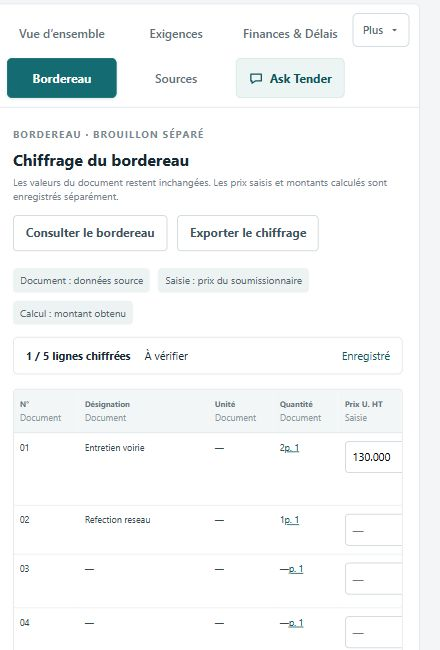
\includegraphics[width=0.59\textwidth]{screenshots/05_pricing_detail.jpg}
\caption{Brouillon de chiffrage sur la même fixture synthétique : origine des valeurs et état « à vérifier » après une saisie divergente.}\label{fig:ui-pricing}
\end{figure}

Le CSV extrait et le CSV de chiffrage sont deux exports séparés. Les champs textuels susceptibles d'être interprétés comme formule par un tableur sont neutralisés. La sauvegarde du brouillon est indépendante de la réponse d'analyse et la revue humaine conserve également sa propre trace. Ce sont des mécanismes de fiabilité d'une démonstration locale ; ils ne remplacent ni une politique de droits ni une procédure de validation des offres.
